\chapter{Density Estimation}
\label{chp:dens}
The probability density function (PDF), $f$, is the statistical distribution of a population that, once determined, allows for the maximum extraction of statistical information about the population. Sometimes the probability density function (PDF) - usually just referred to as the density or density function - of the population can be deduced from the nature of the statistical experiment, however this is not always the case. When the population density is unknown it can be estimated parametrically or non-parametrically. In parametric density estimation data is assumed to follow a given distribution. This distribution is estimated by estimating the relevant parameters for the distribution - e.g. the mean and variance for the normal distribution. In non-parametric density estimation data is allowed to speak for itself and initially no assumptions, besides there existing a PDF, is made. In contrast to the parametric case the non-parametric case does not attempt to estimate parameters of the PDF, but rather the PDF itself. The naive approach is to consider what is called the empirical cumulative distribution function (CDF) defined as follows\citep{scott}
\begin{equation}
	\hat{F}(\vec{x})\equiv \frac{\#\{\vec{x}\leq \vec{x}\}}{n},<\quad\forall \vec{x}\in \mathcal{R}^d.
	\label{eeq1}
\end{equation}
From the CDF the density can be estimated as follows
\begin{equation}
	\begin{split}
		\hat{f}(\vec{x})&\equiv \frac{\partial ^d\hat{F}(\vec{x})}{\partial x_1\partial x_2\dots \partial x_d}=\frac{1}{n}\sum_{i}\delta^d(\vec{x}-\vec{x}_i).
	\end{split}
	\label{eq1}
\end{equation}
However - as is evident from equation \eqref{eq1} - this density estimate is a distribution of delta functions and as such worth little in terms of representing a true density that is continuous. The empirical density estimate is a direct representation of the data sample. For this reason the variability of the estimate between different samples from the same population is large (i.e. the variance is large). In order to obtain a better estimate - which varies less between different samples of the same population - information external to the sample has to be applied. Such information can be requiring continuity of the density, the support of the density or expectation of the rough shape of the density (e.g. based on reviewing a histogram). Assuming the true density is continuous, some amount of smoothing (with respect to the empirical estimate) has to be applied. The smoothing action can be implemented in a many different ways, many of which are useful for facilitating a discussion and fewer of which are in the end expedient to use in estimating the true density. 
\newline
This report will focus on univariate (section \eqref{sec:uni}) and multivariate (section \ref{sec:mul}) density estimation using weight function estimators and especially kernel estimators. It will be of particular interest to derive rules of thumb for the parameters of kernel estimation and test the precision of these in numerical experiments. Since there are many relevant and illuminating numerical experiments to considered, the report is structured such that these are located in the text as examples where relevant. The idea behind this is to have the experiment in the vicinity of the relevant text and not have a disjoint pile of experiments in the end.

\section{Univariate Density Estimation}
\label{sec:uni}
\noindent A first stab at implementing the smoothing action is to apply the two-sided numerical derivative instead of the derivative operator in equation \eqref{eq1}. By doing so the (univariate) density estimate is given by
\begin{equation}
	\hat{f}(x)=\frac{\hat{F}(x+\frac{h}{2})-\hat{F}(x-\frac{h}{2})}{h},
	\label{eeq2}
\end{equation} 
where $h$ is a smoothing parameter.
\begin{example}
	\noindent Figure \ref{fig:1a} shows a histogram and plots of the CDF and PDF - using equation \eqref{eeq1} and \eqref{eeq2}, respectively - of the treatment data from \citep{silverman}.
	
	\begin{figure}[H]
		\centering
		\captionsetup{width=0.95\textwidth}
		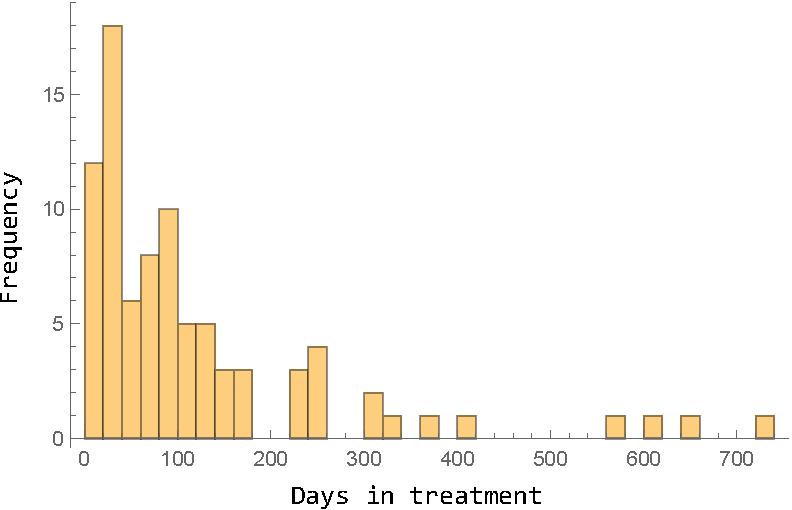
\includegraphics[width=0.32\textwidth]{figures/P3.pdf}
		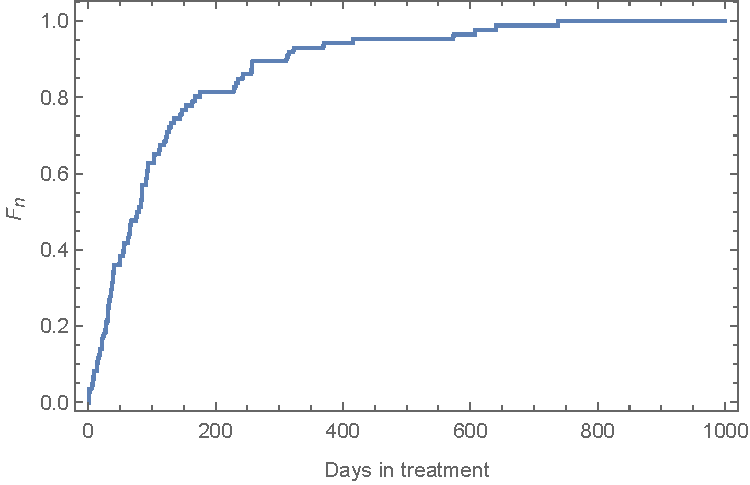
\includegraphics[width=0.32\textwidth]{figures/P4.pdf}
		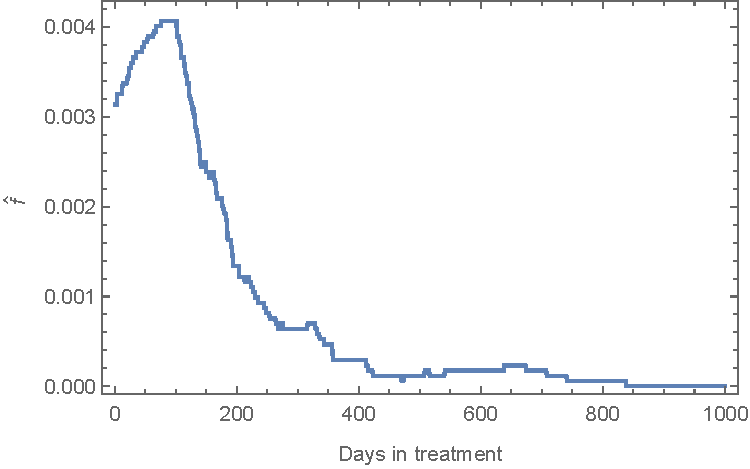
\includegraphics[width=0.32\textwidth]{figures/P5.pdf}
		\caption
		{Left: Histogram of the treatment data (50 bins). Middle: Empirical CDF of the treatment data. Right: Density estimate computed via equation \eqref{eeq2} with $h=200$ chosen subjectively.}
		\label{fig:1a}
	\end{figure}
\end{example}
The above example illustrates the smoothing action of the two-sided numerical derivative relative to the derivative operator (a collection of delta functions). The smoothing by the two-sided derivative is equivalent to sliding a rectangular kernel (of width $h$) across the data and computing the average within the rectangle as it moves across data. This approach can be generalized to the class of estimators called general weight function estimators; let $w(x,y)$ be a function which satisfy
\begin{equation}
	\int_{-\infty }^{\infty}dy w(x,y)=1
\end{equation}
with
\begin{equation}
	w(x,y)\geq 0 \quad \forall x,y.
\end{equation}
The general weight function estimators are then defined, in terms of $w$, viz\citep{silverman}
\begin{equation}
	\hat{f}(t)=\frac{1}{n}\sum_{i=1}^nw(x_i,t).
	\label{we}
\end{equation}
The degree and implementation of the smoothing action is controlled by the function $w$. Table \ref{t1} list some common classes of $w$.
\begin{center}
	\begin{tabular}{ l| c }
		Estimator & $w$  \\
		\hline
		Histogram & $w(x,y)=\begin{cases}
			h^{-1}(x) \quad &\text{if x and y fall in the same bin}\\
			0&\text{Otherwise}
		\end{cases}$ \\
		Orthogonal series & $w(x,y)=\sum_{\nu=0}^{\Lambda}\phi_\nu(x)\phi_\nu(y)$ \\
		Kernel & $w(x,y)=\frac{1}{h}K\big(\frac{y-x}{h}\big)$ \\
		Generalized $k$'th nearest neighbor & $w(x,y)=\frac{1}{d_k(t)}K\big(\frac{y-x}{d_k(t)}\big)$ \\
	\end{tabular}
	\captionsetup{width=0.9\textwidth}
	\captionof{table}{} 
	\label{t1}
\end{center}
In relation to table \ref{t1}; $\Lambda$ is a cutoff that determines the amount of smoothing and $d_k(t)$ is the Euclidean distance to the $k$'th nearest point from $t$. Each weight function smooths the data in a different way and has different strengths/weaknesses. The histogram provides an easy, intuitive representation of data, however, this estimate contains discontinuities and has a high dependence on the sampled data. Hence, as far as estimating the true density, the histogram is rather wanting. The orthogonal series method estimates the probability density via developing it from a set of basis functions. The basis functions depend on the support of the density function. In general, when the real line $(-\infty,\infty)$ or half the real line $[0,\infty)$ are the support, Hermite and Laguerre series are recommended\citep{Efromovich}. If, on the other hand, the density function has a compact support $[0,1]$, then a Fourier series can be used\citep{silverman}. The drawback of the orthogonal series method is that the density estimate may not be a bona fide probability density, meaning that it may not integrate to unity and it can possibly take on negative values\citep{Efromovich}. The kernel estimate and the generalized $k$'th nearest neighbor estimate are related in that both estimates utilize kernels (see table \ref{t2} for some common\citep{silverman} univariate kernels\footnote{The meaning and derivation of "Efficiency" in Table \ref{t2} is covered later.}). The kernels are usually assumed to have continous derivatives to all required orders and to be symmetric functions satisfying\citep{silverman}
\begin{equation}
	\int dt K(t)=1,\qquad \int dt tK(t)=0\quad \text{and}\quad \int dt t^2K(t)=k_2\neq 0.
	\label{prop}
\end{equation}
From table \ref{t1} it is clear that the difference between the kernel estimate and the $k$'th nearest neighbor estimate lies in the window width applied. For the former a fixed window width is applied whereas for the latter a position dependent window width is used. The fixed window width is less flexible as compared to the position dependent one. The danger associated with increased flexibility is, as discussed previously, that the variance of the estimate can become too high, meaning that the results depend too much on the particular sample of data and by extension the estimate of the true density suffers. The two methods can be combined into the sample-point\footnote{In the sample point adaptive estimators $h\rightarrow h(x_i)$. Alternatively one could let $h\rightarrow h(t)$, which would result in another class of adaptive estimators (not considered in this study).} adaptive estimate. This estimate consists of a series of steps\citep{silverman};
\begin{enumerate}
	\item Develop a pilot estimate $\tilde{f}$ for which $\tilde{f}(x_i)>0$.
	\item Define a local bandwidth, $\lambda_i$ viz
	\begin{equation}
		\lambda_i\equiv \bigg(\frac{g}{\tilde{f}(x_i)}\bigg)^\alpha,
		\label{lam}
	\end{equation}
	where
	\begin{equation}
		g=e^{\frac{1}{n}\sum_{i}ln(\tilde{f}(x_i))}
	\end{equation}
	is the geometric mean of $\tilde{f}$ and $0\leq \alpha\leq 1$ is a sensitivity parameter\footnote{$\alpha=0$ returns the pilot estimate whereas $\alpha=1$ is the generalized nearest neighbor estimate.}. 
	\item The adaptive estimate is then (for the univariate case) defined  by letting $h\rightarrow h\lambda_i$ in the kernel estimate. That is
	\begin{equation}
		\hat{f}(t)=\frac{1}{n}\sum_{i}\frac{1}{h\lambda_i}K\bigg(\frac{t-x_i}{h\lambda_i}\bigg).
	\end{equation}
\end{enumerate}
The adaptive estimate is relatively insensitive of the pilot estimate and so it is expedient to use a pilot estimate that provides both low computation time and analytical complexity.
\begin{center}
	\begin{tabular}{ l| c r}
		Kernel & $K(t)$ & Efficiency \\
		\hline
		Epanechnikov & $\begin{cases}
			\frac{3}{4\sqrt{5}}(1-\frac{1}{5}t^2)&\quad \text{for } |t|<\sqrt{5}\\
			0&\quad \text{Otherwise}\\
		\end{cases}$  & $1$\\
		Biweight & $\begin{cases}
			\frac{15}{16}(1-t^2)^2&\quad \text{for } |t|<1\\
			0&\quad \text{Otherwise}\\
		\end{cases}$  & $0.9939$\\
		Triangular & $\begin{cases}
			1-|t|&\quad \text{for } |t|<1\\
			0&\quad \text{Otherwise}\\
		\end{cases}$  & $0.9859$\\
		Gaussian & $\frac{e^{-\frac{t^2}{2}}}{\sqrt{2\pi}}$  & $0.9512$\\
		Rectangular & $\begin{cases}
			\frac{1}{2}&\quad \text{for } |t|<1\\
			0&\quad \text{Otherwise}\\
		\end{cases}$  & $0.9295$\\
	\end{tabular}
	\captionsetup{width=0.95\textwidth}
	\captionof{table}{} 
	\label{t2}
\end{center}
\begin{example}
	\noindent The treatment data from \citep{silverman} denotes the number of days a set of test persons spent in treatment. Hence, the possible values are positive integers. The true density will reflect this parameter space and vanish below $1$. In order to make an accurate density estimate the kernel should reflect this property as well. Naively applying the kernels of Table \ref{t2} will result in a density estimate yielding a finite probability of negative days in treatment. The issue can be alleviated by transforming data such that the distribution more closely resembles the kernel function. After the transformation the data can be transformed back and so a density estimate featuring this central property of the true density can be obtained in this way. The sequence can be captured in one operation by using
	\begin{equation}
		f(t)dt=f(a(t))da(t)\Rightarrow f(t)=f(a)d_ta,
	\end{equation}
	where $a$ is any transformation of the data, e.g. $a(t)=ln(t)$. Note however that both $t\rightarrow a(t)$ and $x_i\rightarrow a(x_i)$ in the transformation. For the treatment data it is expedient to perform a log-transformation of data. This results - for the Gaussian, Epanechnikov and rectangular kernels - in the density estimates
	\begin{equation}
		\begin{split}
			\text{Gaussian kernel:}&\quad\hat{f}(t)=\frac{1}{n}\sum_{i=1}^n\frac{1}{ht}\frac{1}{\sqrt{2\pi }}e^{-\frac{1}{2}\big(\frac{ln(t)-ln(x_i)}{h}\big)^2},\\
			\text{Epanechnikov kernel:}&\quad\hat{f}(t)=\frac{1}{n}\sum_{i=1}^n\begin{cases}
				\frac{1}{ht}\frac{3}{4\sqrt{5}}\bigg(1-\frac{1}{5}\big(\frac{ln(t)-ln(x_i)}{h}\big)^2\bigg)&\quad \text{for } \big|\frac{ln(t)-ln(x_i)}{h}\big|<\sqrt{5}\\
				0&\quad \text{Otherwise}\\
			\end{cases},\\
			\text{Rectangular kernel:}&\quad\hat{f}(t)=\frac{1}{n}\sum_{i=1}^n\begin{cases}
				\frac{1}{2ht}&\quad \text{for } \big|\frac{ln(t)-ln(x_i)}{h}\big|<1\\
				0&\quad \text{Otherwise}\\
			\end{cases}.\\
		\end{split}
	\end{equation}
	The density estimates using the Gaussian, Epanechnikov and rectangular kernels as well as the log-transformed estimates of the three and the adaptive Gaussian kernel are shown in figure \ref{fig:1}. From the figure it is clear how the non-log-transformed estimates predict a non-vanishing probability for negative days in treatment and how this is not the case for the log-transformed estimates. From the figure it is also clear that the density estimates using different kernels are quite similar, although the density estimates using the rectangular kernel window is noisy relative to the others.
	\begin{figure}[H]
		\centering
		\captionsetup{width=0.95\textwidth}
		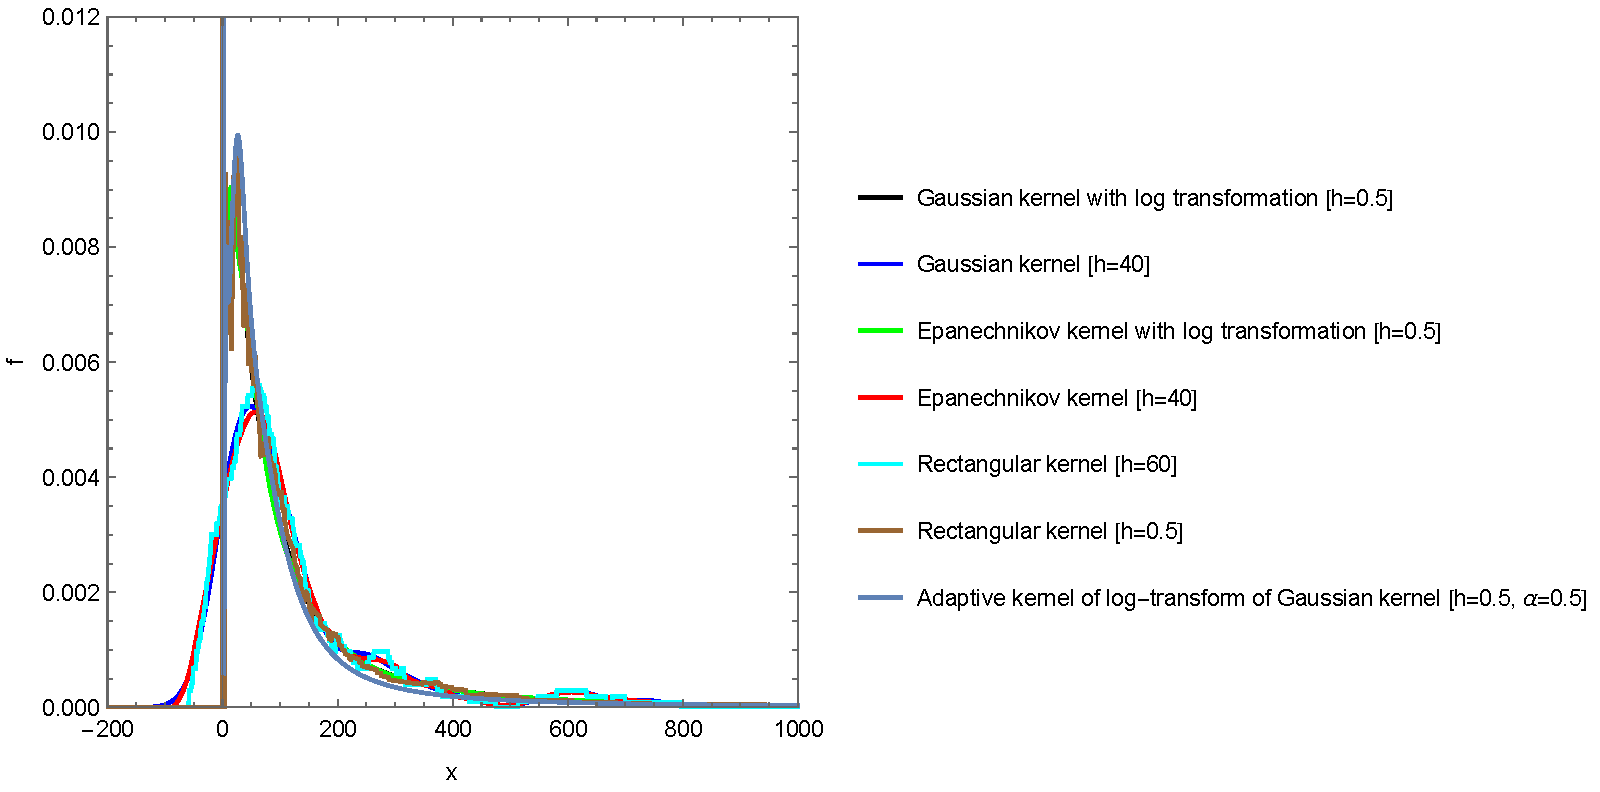
\includegraphics[width=0.8\textwidth]{figures/P11.pdf}
		\caption{}
		\label{fig:1}
	\end{figure}
\end{example}
\noindent Example 1.2 illustrate two challenges in density estimation, namely determining the smoothing parameter ($h$) and - in the case of the adaptive estimate - also the sensitivity parameter ($\alpha$). Intuitively it is expected that the optimal values of $h$ and $\alpha$ should depend on the true density - that is information not contained in the sample. This argument goes in favor of choosing $\alpha$ and $h$ subjectively based on expectations and knowledge external to the sample. That being said it is useful to be aware of the optimal values for $h$ and $\alpha$ given some assumptions and use these as rules of thumb. 

\subsection{Determining the parameters of density estimation}
The parameters of density estimation ($h,\alpha$) are conventionally determined such that the difference between the true density $f$ and the density estimate $\hat{f}$ is minimized. There exist many measures of difference between density distributions. In this study the total variation (TV), Kullback-Leibler divergence and mean integrated squared error (MISE) will be considered.
\begin{equation}
	\begin{split}
		TV(f,\hat{f})&=\frac{1}{2}\int |\hat{f}(x)-f(x)|dx,\\
		I(f,\hat{f})&=\int f(x)\log\bigg(\frac{f(x)}{\hat{f}(x)}\bigg)dx,\\
		MISE[f,\hat{f}]&= \mathbb{E}\bigg[\int(\hat{f}(x)-f(x))^2\bigg]dx.\\
	\end{split}
\end{equation}
The TV is the largest possible difference between predicted probabilities of two probability distributions. Because of this nice, intuitive interpretation the TV is used to evaluate the numerical experiments conducted in this study. However, there is no simple way of estimating the TV, so a different, somewhat equivalent, measure (of which there are many) is considered for the analytical manipulation associated to parameter determination; the Kullback-Leibler (KL) divergence. This is the procedure used in the maximum likelihood approach to parameter estimation. The two measures are related via the Pinsker inequality
\begin{equation}
	TV(f,\hat{f})\leq \sqrt{\frac{1}{2}I(f,\hat{f})},
	\label{Pinsker}
\end{equation}
from which it is clear that minimizing the Kullback-Leibler divergence will result in a minimization of the TV as well. The last probability measure considered is the MISE. The MISE has the advantage of being (relatively) analytically forgiving however, it does not have the same intuitive probabilistic interpretation as the TV.

\subsubsection{Parameter Estimation via the MISE}
Parameter estimation via the MISE is (evidently) centered around the MISE, given by
\begin{equation}
	\begin{split}
		MISE[f,\hat{f}]&\equiv \mathbb{E}\bigg[\int_{-\infty}^{\infty} (\hat{f}(x)-f(x))^2dx\bigg]\\
		&= \int_{-\infty}^{\infty} MSE_x[\hat{f}]dx\bigg]\\
		&= \int_{-\infty}^{\infty} (\mathbb{E}[\hat{f}(x)]-f(x))^2dx+\int_{-\infty}^{\infty}Var[\hat{f}(x)]dx,\\
	\end{split}
	\label{mse1}
\end{equation}
where
\begin{equation}
	\begin{split}
		MSE_x[f,\hat{f}]&\equiv \mathbb{E}[(\hat{f}(x)-f(x))^2]\\
		&=(\mathbb{E}[\hat{f}(x)]-f(x))^2+Var[\hat{f}(x)].
	\end{split}
\end{equation}
Using the MISE for parameter estimation conventionally proceed via one of two different routes; i) expand the bias and variance in the smoothing parameter ($h$) and determine the parameters that minimize the asymptotic limit ($h\rightarrow 0\wedge  n\rightarrow \infty$) of the MISE ii) estimate the MISE itself from data and iteratively determine the values of $h,\alpha$ that minimize the estimated MISE.  

\paragraph{Route 1: The asymptotic MISE}
In route one the asymptotic limit ($h\rightarrow 0\wedge  n\rightarrow \infty$) of the MISE is considered and the parameters are chosen in order to minimize this limit. The regular (non-adaptive) estimate can be considered as the limit of $\alpha\rightarrow 0$ of the adaptive estimate, so it will suffice to consider the expansion of the adaptive estimate.\newline
In line with the short description of the asymptotic limit above the straightforward approach would be to perform an expansion of the bias and variance (with $h\rightarrow 0\wedge  n\rightarrow \infty$) to leading order and set the sensitivity and smoothing parameters such that the asymptotic MISE (AMISE) is minimized. However, it turns out that the leading order in the bias can be eliminated by a particular choice of the sensitivity parameter, namely $\alpha=\frac{1}{2}$. For this reason $\alpha=\frac{1}{2}$ can be used as a rule of thumb for the sensitivity parameter\citep{silverman}. However, by eliminating the leading order of the bias, there cannot be an associated rule of thumb for\footnote{Because the next to leading order leads to unbounded integrals for this choice of $\alpha$.} $h$, and so one is left with choosing $h$ subjectively or using an unrelated rule of thumb. An alternative approach is to pick $\alpha$ to eliminate the next to leading order term in the bias ($\alpha=\frac{1}{4}$) and then pick $h$ to minimize the AMISE. This strategy results in a relevant rule of thumb for $h$ and is further motivated by the fact that the higher order terms in the bias expansion are - in general - significant in magnitude. Motivated by the notion that the higher order terms of the bias are relevant, one can also try to pick the sensitivity parameter to minimize the entire bias to all orders under the assumption that - apart from the factorized numerical coefficient and dependence on $\alpha$ - all orders are of the similar magnitude ($\alpha \simeq 0.55$). However (as is the case for $\alpha=\frac{1}{2})$, this choice of sensitivity parameter leads to unbounded integrals in the leading order of the bias and so there is no associated rule of thumb for $h$ in this case either. Adding this on top of the strong assumption on the magnitude of all orders in the bias expansion makes this last choice not recommended based on the arguments presented here. However, it goes to show that taking $\alpha\sim 0.5$ possibly also reduce the higher order terms in the bias - on top of eliminating the leading order. Hence, based on the arguments presented here, $\alpha\sim 0.5$ would seem the best choice for the sensitivity parameter given a rule of thumb on $h$ is of no interest. However, as it turns out, the difference between taking $\alpha=\frac{1}{4}$ and $\alpha=\frac{1}{2}$ is very small in the numerical examples later considered and so taking $\alpha=\frac{1}{4}$ with the associated rule of thumb for $h$ emerge as the recommended strategy. For the examples considered in one dimension, this strategy proves very effective.\newline\newline
\noindent To provide details on the above outline, begin with examining the bias for the adaptive estimate in the univariate case, or - to the same end - the expectation value for the adaptive estimate
\begin{equation}
	\begin{split}
		\mathbb{E}[\hat{f}(t)]&=\frac{1}{n}\sum_i\mathbb{E}[w(x_i,t)]\\
		&=\frac{1}{h}\int_{-\infty}^{\infty} dx f(x)^{\alpha+1} K\bigg(\frac{t-x}{h}f(x)^\alpha\bigg)\\
		&=\int_{-\infty}^{\infty} du f(t+hu)^{\alpha+1} K\big(uf(t+hu)^\alpha\big),\\
	\end{split}
	\label{b1}
\end{equation}
where $u=\frac{x-t}{h}$ and the symmetry of the kernel has been used in going from line one to two. Following \citep{silverman} $g=1$ is assumed in choosing the smoothing and sensitivity parameters. Taylor expanding the integrand reveals (see appendix \ref{app1})
\begin{equation}
	\begin{split}
		\mathbb{E}[\hat{f}]=&f+(1-2\alpha)\frac{h^2}{2f^{2\alpha+1}}\int_{-\infty}^{\infty} da a^2K(a)\big[f\partial_t^2f-2\alpha(\partial_tf)^2\big]\\
		&-(1-4\alpha)\frac{h^4}{24f^{4\alpha +3}}\int_{-\infty}^{\infty} da a^4 K(a)\big[8\alpha(2\alpha+1)(4\alpha+1)(\partial_tf)^4\\
		&\qquad\qquad\qquad\qquad\qquad\qquad\qquad+4\alpha f[4f\partial_tf \partial_t^3f-18(4\alpha-1)(\partial_tf)^2\partial_t^2f\\
		&\qquad\qquad\qquad\qquad\qquad\qquad\qquad\qquad\quad+3f(\partial_t^2f)^2]-f^3\partial_t^4f
		\big]+\mathcal{O}(h^5).
	\end{split}
	\label{b22}
\end{equation}
As is clear from equation \eqref{b22}; taking $\alpha=\frac{1}{i}$ will eliminate the $\mathcal{O}(h^i)$ term. As mentioned previously; it is often assumed that the leading order is the dominating one and so $\alpha=\frac{1}{2}$ can be suggested as a rule of thumb\citep{silverman}. However, the $\mathcal{O}(h^4)$ term is significant (it often dominate) in the $h$-$\alpha$ plane of the bias for even moderate values of $\alpha$ and so it is expedient to instead take, as a rule of thumb, $\alpha=\frac{1}{4}$ such that the higher order term is eliminated. The fact that the higher order term in the bias dominate the choice of $\alpha$ indicate that even higher orders in the bias may be relevant. Considering now only the factorized numerical coefficients and $\alpha$ - let the rest be $\sim\mathcal{O}(1)$ for all orders for simplicity. In this case the integrated squared bias will have the form
\begin{equation}
	\begin{split}
		\int_{-\infty}^{\infty}(\mathbb{E}[\hat{f}]-f)^2dx&\sim \bigg(\sum_{i=1}^{\infty}\frac{(1-2i\alpha)(-1)^i}{(2i)!}\bigg)^2\\
		&=(cos(1)+\alpha sin(1)-1)^2
	\end{split}
	\label{bias}
\end{equation}
Equation \eqref{bias} is minimized for $\alpha=0.546\simeq 0.55$. This value for $\alpha$ relies on the strict requirement that all orders in the expansion of the bias - apart from the factorized numerical coefficients and $\alpha$ - are of the same order. Moving on to the variance
\begin{equation}
	\begin{split}
		Var[\hat{f}(t)]&=\frac{1}{n}\sum_iVar[w(x_i,t)]\\
		&=\frac{1}{n}\bigg[\frac{1}{h^2}\int_{-\infty}^{\infty}dx K\bigg(\frac{t-x}{h}f(x)^\alpha\bigg)^2f(x)^{2\alpha+1}-\bigg(\frac{1}{h}\int_{-\infty}^{\infty}dxK\bigg(\frac{t-x}{h}f(x)^\alpha\bigg)f(x)^{\alpha+1}\bigg)^2\bigg]\\
		&=\frac{1}{n}\bigg[\frac{1}{h}\int_{-\infty}^{\infty}du K\big(uf(t+hu)^\alpha\big)f(t+hu)^{2\alpha+1}+\mathcal{O}(h^0)\bigg]\\
		&=\frac{f(t)^{\alpha+1}}{nh}\int_{-\infty}^{\infty}da K(a)^2+\mathcal{O}(n^{-1})\\
	\end{split}
\end{equation}
Implicitly taking $\alpha=\frac{1}{4}$ (and hereby assuming the $\mathcal{O}(h^2)$ term in the bias dominate) the AMISE can be written
\begin{equation}
	AMISE[\hat{f}]= (1-2\alpha)^2\frac{h^4k_2^2}{4}\int_{-\infty}^{\infty}dx\bigg(\frac{f\partial_t^2f-2\alpha(\partial_tf)^2}{f^{2\alpha+1}}\bigg)^2+\frac{1}{nh}\int_{-\infty}^{\infty}dxf^{\alpha+1}\int_{-\infty}^{\infty}da K^2,
	\label{mise2}
\end{equation}
where the arguments are suppressed and the regular AMISE is obtained by setting $\alpha=0$. Equation \eqref{mise2} illustrates what is often referred to as the bias-variance trade off; $\lim\limits_{h\rightarrow 0}(bias)=0$ however $\lim\limits_{h\rightarrow 0}(variance)=\infty$ and vice versa for $h\rightarrow \infty$. Hence, there is a trade off between the bias and variance. The value of $h$ that minimize the AMISE is referred to as the optimal $h$. In the case of equation \eqref{mise2}, it is given by
\begin{equation}
	h_{opt}= \bigg(\frac{\int_{-\infty}^{\infty}dxf^{\alpha+1}\int_{-\infty}^{\infty}da K^2}{(1-2\alpha)^2nk_2^2\int_{-\infty}^{\infty}dx\big(f^{-(2\alpha+1)}[f\partial_t^2f-2\alpha(\partial_tf)^2]\big)^2}\bigg)^\frac{1}{5}.
	\label{h3}
\end{equation}
Equation \eqref{h3} illustrates that the optimal value for $h$ depends on the true $f$. It is also clear that $\lim\limits_{n\rightarrow \infty}(h_{opt})=0$, however this limit is approached at a slow rate. Because the optimal value of the smoothing parameter depends on the true density there is no standard choice of $h$ that is ideal for all possible true densities (beyond rules of thumb). Conventionally a subjective pick of $h$ is taken based on the expectations of the true distribution. If the true distribution is known a better estimate can be computed. A rule of thumb is to reference the case where $f\sim\mathcal{N}$ and parametrize the dependence on the kernel viz
\begin{equation}
	B(K)=\bigg(\frac{\int_{-\infty}^{\infty}da K(a)^2}{(\int_{-\infty}^{\infty}dxx^2K(x))}\bigg)^\frac{1}{5}.
\end{equation}
$h_{opt}$ - derived based on the leading order in the expansion of the bias - for different values of $\alpha$ is shown in table \ref{t4} in the second column. In the third column adjusted values of $h_{opt}$ is listed. The adjustment of $h_{opt}$ is heuristically motivated such that the best estimate across true densities is obtained\citep{silverman}. The adjusted $h_{opt}$ in the first row is taken directly from \citep{silverman} whereas the adjusted $h_{opt}$ in the second row is derived from inspiration of the former. 
\begin{center}
	\begin{tabular}{ l|| c| c|}
		$\alpha$ & $h_{opt}(f,K\sim \mathcal{N})$  & Adjusted $h_{opt}(f,K\sim \mathcal{N})$\\
		\hline
		$0$ & $1.37\hat{\sigma} n^{-\frac{1}{5}}B(K)$ & $1.17\min\big(\hat{\sigma},\frac{\hat{R}}{1.34}\big)n^{-\frac{1}{5}}B(K)$ \\
		$1/4$ & $1.30\hat{\sigma}^\frac{3}{4}n^{-\frac{1}{5}}B(K)$ & $1.11\min\big(\hat{\sigma}^\frac{3}{4},\big(\frac{\hat{R}}{1.34}\big)^\frac{3}{4}\big)n^{-\frac{1}{5}}B(K)$ \\
		$1/2$ & NA&  NA\\
		$0.55$ &  NA & NA \\
	\end{tabular}
	\captionsetup{width=0.95\textwidth}
	\captionof{table}{$\min(x,y)$ picks the smaller of the two quantities, $\hat{\sigma}$ is the estimate of the standard deviation of the true normal distribution and $\hat{R}$ is the estimate of the interquartile range.} 
	\label{t4}
\end{center}
Substituting $h_{opt}$ from equation \eqref{h3} back into the AMISE yields
\begin{equation}
	AMISE[\hat{f}]= \frac{5}{4}C(K)\bigg(\int_{-\infty}^{\infty}dxf^{\alpha+1}\bigg)^\frac{4}{5}\bigg(\frac{(1-2\alpha)^2}{n^4}\int_{-\infty}^{\infty}dx\bigg(\frac{f\partial_t^2f-2\alpha(\partial_tf)^2}{f^{2\alpha+1}}\bigg)^2\bigg)^\frac{1}{5},
	\label{mise3}
\end{equation}
where
\begin{equation}
	C(K)=\bigg(\sqrt{k_2}\int_{-\infty}^{\infty}dt K(t)^2\bigg)^{\frac{4}{5}}.
	\label{ck}
\end{equation}
Equation \eqref{mise3} illustrates that $K$ should be chosen such that $C(K)$ is small. \citep{silverman} shows that $C(K)$ is minimized by the Epanechnikov kernel. The efficiency of a kernel is therefore defined with respect to the Epanechnikov kernel. Denote the Epanechnikov kernel by $K_e$, then the efficiency is defined as
\begin{equation}
	\begin{split}
		eff(K)&\equiv \bigg(\frac{C(K_e)}{C(K)}\bigg)^{\frac{5}{4}}\\
		&=\frac{3}{5\sqrt{5}}\bigg[\frac{1}{\sqrt{\int_{-\infty}^{\infty}dt K(t)t^2}\int_{-\infty}^{\infty}dt' K(t')^2}\bigg].
	\end{split}
\end{equation}
The efficiency is listed alongside the kernels considered in table \ref{t2}.


\paragraph{Route 2: Estimating the MISE}
In route two the MISE itself is estimated from the information in the sample and subsequently minimized with respect to $h,\alpha$. Writing out the MISE
\begin{equation}
	\begin{split}
		MISE[\hat{f}]&\equiv \mathbb{E}\bigg[\int_{-\infty}^{\infty}dx (\hat{f}(x)-f(x))^2\bigg]\\
		&=\int_{-\infty}^{\infty}dx\hat{f}(x)^2-2\int_{-\infty}^{\infty}dxf(x)\hat{f}(x)+\int_{-\infty}^{\infty}dxf(x)^2\\
		&\equiv R(\hat{f},f)+\int_{-\infty}^{\infty}dxf(x)^2,
	\end{split}
	\label{mse4}
\end{equation}
where the last line define $R(\hat{f},f)$. $f$ does not depend on $h,\alpha$, so in this context minimizing $R$ corresponds to minimizing the MISE. The first integral in $R$ is straightforward to write out whereas the second can be estimated by the mean cross-validated estimate of $f$, that is\citep{silverman}
\begin{equation}
	\begin{split}
		\hat{R}(h,\alpha)=\int_{-\infty}^{\infty}dx \bigg[\frac{1}{n}\sum_{i}\frac{1}{h\lambda_i}K\bigg(\frac{x-x_i}{h\lambda_i}\bigg)\bigg]^2-\frac{2}{n}\sum_{i}\hat{f}_{-i}(x_i),
	\end{split}
	\label{r1}
\end{equation}
where the dependence on $\alpha$ is implicit through $\lambda_i$ (see equation \eqref{lam}) and
\begin{equation}
	\hat{f}_{-i}(x_i)=\frac{1}{(n-1)}\sum_{j\neq i}\frac{1}{h\lambda_j}K\bigg(\frac{x_i-x_j}{h\lambda_j}\bigg).
\end{equation}
To see that the latter term in equation \eqref{r1} is a reasonable estimate of the latter integral in $R$, consider the expectation value of the estimator
\begin{equation}
	\begin{split}
		\mathbb{E}\bigg[\frac{1}{n}\sum_{i}\hat{f}_{-i}(x_i)\bigg]&=\mathbb{E}[\hat{f}_{-i}(x_i)]\\
		&=\int \hat{f}(x)f(x)dx.
	\end{split}
\end{equation}
Hence, from equation \eqref{r1} $h,\alpha$ can be determined by numerically minimizing $\hat{R}$. 

\subsubsection{Parameter Estimation via the Kullback-Leibler Divergence}
As mentioned previously, the Kullback-Leibler divergence is connected via to the TV via the Pinsker inequality (equation \eqref{Pinsker}) and so minimizing the Kullback-Leibler divergence yields estimates of the parameters that also minimize the TV. The Kullback-Leibler divergence can be estimated viz
\begin{equation}
	\hat{I}(h,\alpha)=\frac{1}{n}\sum_{i}\log\big(\hat{f}_{-i}(x_i)\big).
	\label{I}
\end{equation}
The expectation of $\hat{I}$ is
\begin{equation}
	\begin{split}
		\mathbb{E}[\hat{I}]&=\mathbb{E}[\log\big(\hat{f}_{-i}(x_i)\big)]\\
		&\simeq\int f(x)\log\big(\hat{f}(x)\big)\\
		&=-I(f,\hat{f})+\int f(x)\log\big(f(x)\big)dx,
	\end{split}
	\label{in}
\end{equation}
where the approximation lies in letting the estimate of $f$ based on $n-1$ observations go to the estimate of $f$ based on $n$ observations (i.e. let $\hat{f}_{-i}\rightarrow \hat{f}$). Equation \eqref{in} shows that $\hat{I}$ is an unbiased estimator of $I$ up to a constant. Hence, from equation \eqref{I} $h,\alpha$ can be determined by numerically minimizing $\hat{I}$.

\section{Multivariate Density Estimation}
\label{sec:mul}
\noindent The generalization of the univariate formalism to the multivariate case proceeds by generalizing the kernel and accounting for the possibility of the different variables having different scales. The latter can be accounted for by linearly transforming data such that
\begin{equation}
	\hat{f}(\vec{t})=\frac{1}{n |H|}\sum_{i=1}^nK\big(H^{-1}(\vec{t}-\vec{x}_i)\big),
	\label{resc1}
\end{equation}
where $H$ - the smoothing matrix - is a $d\times d$ matrix responsible for the linear transformation of data. The multivariate versions of the Epanechnikov and Gaussian kernels are listed in table\footnote{$c_d$ is the volume of a $d$-dimensional unit-sphere. E.g. $c_1=2$, $c_2=\pi, c_3=\frac{4\pi}{3},\dots$.} \ref{t3}.
\begin{center}
	\begin{tabular}{ l| c }
		Kernel & $K(\vec{w})$ \\
		\hline
		Epanechnikov & $\begin{cases}
			\frac{1}{2c_d}(d+2)(1-\vec{x}^T\vec{x})&\quad \text{for } \vec{x}^T\vec{x}<1\\
			0&\quad \text{Otherwise}\\
		\end{cases}$ \\
		Gaussian & $\frac{e^{-\frac{\vec{x}^T\vec{x}}{2}}}{(2\pi)^\frac{d}{2}}$ \\
	\end{tabular}
	\captionsetup{width=0.95\textwidth}
	\captionof{table}{} 
	\label{t3}
\end{center}
Similarly to the conditions in equation \eqref{prop} the multivariate kernels (considered here) are required to satisfy\citep{scott}
\begin{equation}
	\int_{\mathcal{R}^d} K(\vec{w})d\vec{w}=1,\qquad \int_{\mathcal{R}^d} \vec{w}K(\vec{w})d\vec{w}=\vec{0},\qquad \int_{\mathcal{R}^d} \vec{w}\vec{w}^TK(\vec{w})d\vec{w}=\tilde{k}_2\mathbb{1},
	\label{prop2}
\end{equation}
where $d\vec{x}=dx_1dx_2\dots dx_d$ and $\tilde{k}_2$ is a scalar. The fixed kernel methods generalize to the adaptive kernel method analogously to the univariate case, so again it is a three-step procedure
\begin{enumerate}
	\item Develop a pilot estimate $\tilde{f}$ for which $\tilde{f}(\vec{x}_i)>0$.
	\item Define a local bandwidth, $\lambda_i$ viz
	\begin{equation}
		\lambda_i\equiv \bigg(\frac{g}{\tilde{f}(\vec{x}_i)}\bigg)^\alpha,
	\end{equation}
	where
	\begin{equation}
		g=e^{\frac{1}{n}\sum_{i}ln(\tilde{f}(\vec{x}_i))}
	\end{equation}
	is the geometric mean of $\tilde{f}$.
	\item The adaptive kernel estimate is then (for the multivariate case) 
	\begin{equation}
		\hat{f}(\vec{t})=\frac{1}{n|H|}\sum_{i=1}^n(\lambda_i)^{-d}K\big(\lambda_i^{-1}H^{-1}(\vec{t}-\vec{x}_i)\big),
		\label{rescaled2}
	\end{equation}
	where again the regular estimate is obtained by taking $\alpha\rightarrow 0$.
\end{enumerate}

\subsection{Determining the parameters of density estimation}
The parameters of density estimation in the multivariate case are determined analogously to the univariate case. In this study the generalized versions of the total variation (TV), Kullback-Leibler divergence and mean integrated squared error (MISE) will be considered.
\begin{equation}
	\begin{split}
		TV(f,\hat{f})&=\frac{1}{2}\int_{\mathcal{R}^d} |\hat{f}(\vec{x})-f(\vec{x})|d\vec{x},\\
		I(f,\hat{f})&=\int_{\mathcal{R}^d} f(\vec{x})\log\bigg(\frac{f(\vec{x})}{\hat{f}(\vec{x})}\bigg)d\vec{x},\\
		MISE[f,\hat{f}]&= \mathbb{E}\bigg[\int_{\mathcal{R}^d}(\hat{f}(\vec{x})-f(\vec{x}))^2\bigg]d\vec{x},\\
	\end{split}
\end{equation}
where again the TV and Kullback-Leibler divergence is related via the Pinsker inequality (equation \eqref{Pinsker}).

\subsubsection{Parameter Estimation via the MISE}
Using the MISE the parameter estimation proceeds completely analogously to the univariate case via one of two different routes; i) expand the bias and variance in the smoothing parameter ($h$) and determine the parameters that minimize the asymptotic limit ($h\rightarrow 0\wedge  n\rightarrow \infty$) of the MISE ii) estimate the MISE itself from data and iteratively determine the values of $h,\alpha$ that minimize the estimated MISE. The only difference is the challenge and changes that come from the multivariate formalism.  

\paragraph{Route 1: The asymptotic MISE}
The first route proceeds analogous to the univariate case. The asymptotic expansion shows that in general (see appendix \ref{app:exp})
\begin{equation}
	\mathbb{E}[\hat{f}]-f=\sum_{i=1}^{\infty}\frac{1-[2i+1-d]\alpha}{(2i)!}\cdot (\dots).
	\label{do}
\end{equation}
Hence - in accordance with the results from the univariate case - the $i$'th term in the bias can be eliminated by setting $\alpha=\frac{1}{2i+1-d}$. Similarly to the univariate case $\alpha$ can be set to eliminate the leading order or the next to leading order. Contrary to eliminating the leading order, eliminating the next to leading order will result in an associated rule of thumb for $h$ - giving this choice a competitive advantage. Letting $(\dots)$ in equation \eqref{do} be of the same order for $d=1$ results in the bias being minimized for $\alpha\simeq 0.55$ as found in the univariate case. For $d\geq 2$ however, this procedure reveals $\alpha>1$ and so is not a viable option in this case. Hence, the options remain to eliminate either the leading or next to leading order in the bias. The difference between the two choices of $\alpha$ is little - as seen in the univariate case - and so the choice resulting in an associated rule of thumb value for $h$ may be favoured for just this reason.\newline\newline
\noindent For the multivariate adaptive estimate the smoothing matrix and sensitivity parameter are - analogously to the univariate case - determined by investigating the asymptotic expansion of the MISE. The expectation value in this case (see appendix \ref{app:exp})
\begin{equation}
	\mathbb{E}[\hat{f}]=f+\frac{[1-(3-d)\alpha]\tilde{k}_2}{2}\bigg[\frac{fTr[H^T\tau H]-(3-d)\alpha Tr[H^T\Lambda H]}{f^{2\alpha+1}}\bigg]+\mathcal{O}(H^3),
\end{equation}
where $\tau_{jk}=\frac{\partial^2 f}{\partial t_j\partial t_k}$ and $\Lambda_{jk}=\frac{\partial f}{\partial t_j}\frac{\partial f}{\partial t_k}$. The variance term is computed straightforwardly and so the AMISE is
\begin{equation}
	\begin{split}
		AMISE[\hat{f}]=& [1-(3-d)\alpha]^2\frac{\tilde{k_2^2}}{4}\int_{\mathcal{R}^d} \bigg(\frac{fTr[H^T\tau H]-(3-d)\alpha Tr[H^T\Lambda H]}{f^{2\alpha+1}}\bigg)^2d\vec{x}\\
		&+\frac{1}{n|H|}\int f^{\alpha+1}d\vec{x}  \int_{\mathcal{R}^d} K^2d\vec{w}.
	\end{split}
	\label{mise4}
\end{equation}
Next, parametrize the $H$-matrix viz
\begin{equation}
	H=hA,
	\label{H}
\end{equation}
where $h>0$ is a scalar. Minimizing the AMISE with respect to $h$ reveals
\begin{equation}
	h_{opt}= \bigg[\frac{d}{[1-(3-d)\alpha]^2n|A|}\frac{\int f^{\alpha+1}d\vec{x}  \int_{\mathcal{R}^d} K^2d\vec{w}}{\tilde{k}_2^2\int \big(\frac{fTr[A^T\tau A]-(3-d)\alpha Tr[A^T\Lambda A]}{f^{2\alpha+1}}\big)^2d\vec{x}}\bigg]^{\frac{1}{d+4}}.
	\label{ho1}
\end{equation}
From equation \eqref{ho1} it is clear that - similar to the univariate case - the optimal value for $h$ depends on the true $f$ and again $\lim\limits_{n\rightarrow \infty}(h_{opt})=0$ however at an increasingly slow rate as $d$ increases. In line with the univariate case a rule of thumb value for $h$ is to take $f\sim\mathcal{N}$, $A=\Sigma^\frac{1}{2}$ and defining (see appendix \ref{app:B})
\begin{equation}
	\tilde{B}(K)\equiv \bigg(\frac{\int_{\mathcal{R}^d} K^2d\vec{w}}{\tilde{k}_2^2}\bigg)^\frac{1}{d+4}.
\end{equation} 
$h_{opt}$ - derived based on the leading order in the expansion of the bias (see appendix \ref{app:B}) - for different values of $\alpha$ is shown in table \ref{t5} in the second column. In relation to table \ref{t5} and estimating $h_{opt}$ via a rule of thumb, it is interesting to note that for $d=3$ the procedure of eliminating the next to leading order via $\alpha$ is not possible. For $d=3$ the factorized $\alpha$-dependency of the leading order term vanishes and the next to leading order can be cancelled by setting $\alpha=\frac{1}{2}$. However, for $\alpha=\frac{1}{2}$ the integral in the denominator in $h_{opt}$ diverge and so the next to leading order cannot be canceled in this case. In this case the third leading order term in the bias can be eliminated by setting $\alpha=\frac{1}{4}$ and deriving the associated rule of thumb for $h$ using the leading order.
\begin{center}
	\begin{tabular}{ l|l|l| c|}
		Estimate &$\alpha$ & $d$ & $h_{opt}(f\sim \mathcal{N})$  \\
		\hline
		Regular & $0$ & $d$ & $\big(\frac{4(2\sqrt{\pi})^d}{n(d+2)}\big)^\frac{1}{d+4}\tilde{B}(K)$  \\
		Cancel LO& $\frac{1}{3-d}$ & $d$ & NA\\
		Cancel NTLO &$1/3$ &$2$ & $0.74n^{-\frac{1}{6}}|S|^{-\frac{5}{36}}\tilde{B}(K)$ \\
		Cancel TLO &$1/4$ &$3$ & $0.78n^{-\frac{1}{7}}|S|^{-\frac{5}{56}}\tilde{B}(K)$ \\
	\end{tabular}
	\captionsetup{width=0.95\textwidth}
	\captionof{table}{$|S|$ denotes the determinat of the sample covariance matrix (see e.g. equation \eqref{cov}). LO, NTLO and TLO abbreviates "leading order", "next to leading order" and "third leading order", repsectively and cancel LO, NTLO and TLO denote choosing $\alpha$ chosen to eliminate these terms.} 
	\label{t5}
\end{center}
Substituting $h_{opt}$ from equation \eqref{ho1} back into the AMISE yields
\begin{equation}
	AMISE[\hat{f}]= \frac{d+4}{4d^\frac{d}{d+4}}\tilde{C}(K)\bigg(\frac{\int f^{\alpha+1}d\vec{x} }{|A|n}\bigg)^\frac{4}{d+4}\bigg([1-(3-d)\alpha]^2I_f\bigg)^\frac{d}{d+4}
	,
	\label{misec3}
\end{equation}
where
\begin{equation}
	\tilde{C}(K)\equiv \bigg(\tilde{k}_2^\frac{d}{2}\int_{\mathcal{R}^d} K^2d\vec{w}\bigg)^{\frac{4}{4+d}}, \quad \text{and}\quad I_f\equiv\int \bigg(\frac{fTr[A^T\tau A]-(3-d)\alpha Tr[A^T\Lambda A]}{f^{2\alpha+1}}\bigg)^2d\vec{x}
	\label{cck}
\end{equation}
Similarly to the univariate case the efficiency of kernels can be defined in terms of the Epanechnikov kernel viz
\begin{equation}
	eff(K,d)\equiv \bigg(\frac{\tilde{C}(K_e)}{\tilde{C}(K)}\bigg)^\frac{4+d}{d}.
\end{equation}
Table \ref{t6} shows the efficiency of the Gaussian kernel in table \ref{t3} as a function of dimensionality for $d\in [1,5]$. The decline in $\tilde{C}(K)$ of the Gaussian kernel relative to that of the Epanechnikov kernel is somewhat less than the efficiency, with e.g. $\frac{\tilde{C}(K_e,5)}{\tilde{C}K_G,5)}=0.84$. Since the AMISE is proportional to $\tilde{C}(K)$, the justification for using the Gaussian kernel decrease for increasing $d$, however, with relatively small impact for $d\lesssim 5$. 
\begin{center}
	\begin{tabular}{ l|| c|}
		$d$ & $eff(K_G,d)$ \\
		\hline
		$1$ & $0.95$  \\
		$2$ & $0.89$ \\
		$3$ & $0.82$\\
		$4$ & $0.75$\\
		$5$ & $0.68$\\
	\end{tabular}
	\captionsetup{width=0.95\textwidth}
	\captionof{table}{$eff(K,d)$ for Gaussian kernel in table \ref{t3}.} 
	\label{t6}
\end{center}

\paragraph{Route 2: Estimating the MISE}
Route two proceeds completely analogously to the univariate case. By taking $H=hS^{\frac{1}{2}}$, $\hat{R}$ (with $S$ given by equation \eqref{cov}) can - by straightforward generalization of equation \eqref{r1} - be written
\begin{equation}
	\begin{split}
		\hat{R}(h,\alpha)=\int_{\mathcal{R}^d} \bigg[\frac{1}{nh^d|S|^{\frac{1}{2}}}\sum_{i=1}^n(\lambda_i)^{-d}K\big(\lambda_i^{-1}h^{-1}S^{-\frac{1}{2}}(\vec{t}-\vec{x}_i)\big)\bigg]^2d\vec{y}-\frac{2}{n}\sum_{i}\hat{f}_{-i}(\vec{x}_i),
	\end{split}
	\label{r2}
\end{equation}
now with
\begin{equation}
	\hat{f}_{-i}(\vec{x}_i)=\frac{1}{(n-1)h^d|S|^{\frac{1}{2}}}\sum_{j\neq i}^n(\lambda_i)^{-d}K\big(\lambda_i^{-1}h^{-1}S^{-\frac{1}{2}}(\vec{x}_j-\vec{x}_i)\big).
\end{equation} 
From equation \eqref{r2} $h,\alpha$ can be determined by numerically minimizing $\hat{R}$. 

\subsubsection{Parameter Estimation via the Kullback-Leibler Divergence}
Parameter estimation via the Kullback-Leibler divergernce proceeds by straightforward generalizing the univariate case such that
\begin{equation}
	\hat{I}(h,\alpha)=\frac{1}{n}\sum_{i}\log\big(\hat{f}_{-i}(\vec{x}_i)\big).
	\label{I1}
\end{equation}
From equation \eqref{I1} $h,\alpha$ can be determined by numerically minimizing $\hat{I}$.



\section{Summary}
In this work the formalism of non-parametric density estimation has been introduced and the subject of weight function estimators with associated rules of thumbs for the relevant parameters has been investigated in depth for both the univariate and multivariate case. Several numerical experiments has been conducted, including some which investigate the total variation between different density estimates and the true density. The total variation as a function of sample size for six different distributions has been used to asses the quality of the different density estimates, including a density estimate with approximations of the ideal parameters and density estimates with varying rules of thumbs and approximations of ideal parameter. Such experiments has been conducted thoroughly for one and two dimensional data and - for computational considerations - less thoroughly for three dimensions. The dimensionality has not been increased beyond three because of the computational cost. From the experiments it has been concluded that tuning the sensitivity parameter ($\alpha$) of the adaptive estimates is relatively insignificant next to tuning the smoothing parameter ($h$). For this reason it may be preferential to pick a value of $\alpha$ that come with an associated rule fo thumb value for $h$. It has been shown that the $i$'th order term in $d$ dimensions of the bias is proportional to $\alpha=\frac{1}{2i+1-d}$ in general. There is an associated rule of thumb for $h$ if $\alpha=[0,0.5[$, so as a rule of thumb $\alpha$ can be chosen such to minimize the lowest order in the bias for which this is the case. This strategy (strat1) works well for the univariate case, but less so for the multivariate cases. In the multivariate case it has been shown that choosing $\alpha$ as described above but with the rule of thumb value associated to $\alpha=0$ yields better results (strat2) which, however, only slightly improve upon the results from taking $\alpha=0$ with the associated rule of thumb value (strat3) for $h$ (which is a good pick, especially in the multivariate case). Strat2 seems to improve as dimensionality increases. The reason for this reality has not been investigated in an experiment, but it could be related to the pilot estimate which corresponds to an adaptive estimate with $\alpha=0$. Following \citep{silverman} $g=1$ has been adopted in the AMISE calculations to determine th rule of thumb value for $h$. Taking $g=1$ corresponds to ignoring the uncertainty of the pilot estimate. Hence, it is indicated that this assumption breaks down in $d\geq 2$ and by extension that the uncertainty of the pilot estimate should be accounted for in this case. Doing so is beyond the scope of this study.\newline
Another approach to determine $h,\alpha$ is to estimate the loss function itself from the sample - The Kullback-Leibler divergence has been considered for the univariate as well as multivariate case whereas the MISE has been considered for the univariate case - and minimize it via a grid search. This strategy (strat4) yield good results in the univariate case, especially in case of the Kullback-Leibler divergence. However, in the multivariate case strat4 consistently underperform  with respect to both strat2 and strat3. It is speculated that the underperformance of strat4 in the multivariate case can be alleviated by increasing the amount of points in the grid search used to determine $h,\alpha$. This has not been investigated further as it is beyond the scope of this study; a more in depth study of $TV(n)$ - especially for the multivariate case - requires greater computational power than provided by a common laptop.\newline\newline

\noindent All in all it is concluded that many different strategies do well in the univariate case, with strat1 and strat4 about equally good with strat 3 slightly worse (strat2 has not been tested for the univariate case). For the multivariate case ($2\leq d\leq 3$ has been investigated) strat2 emerge as the best option slightly improving upon strat3. 